\documentclass[11pt,a4paper]{article}

\usepackage[margin=1in, paperwidth=8.3in, paperheight=11.7in]{geometry}
\usepackage{amsmath,amsfonts,fancyhdr,graphicx,caption,subcaption}
\graphicspath{ {img/} }
\usepackage[section,nohyphen]{DomH}
\headertitle{Internet Economics and Financial Technology - Notes}

\begin{document}

\title{Internet Economics and Financial Technology - Notes}
\author{Dom Hutchinson}
\date{\today}
\maketitle

\tableofcontents\newpage

\section{The Big Picture}

\begin{remark}{History of Commercial Computing}
  \begin{itemize}
    \item[\textit{1950-60}] Mainframes - slow; size of rooms.
    \item[\textit{1960-70}] Minicomputers - slow; couple per rooms.
    \item[\textit{1970-80}] PCs - faster; one per desk.
    \item[\textit{1980-90}] LANs - distributed networks.
    \item[\textit{1990-10}] Internet - world wide distributed network.
    \item[\textit{2010-20}] Cloud Computing
  \end{itemize}
  Where does IT go next? Has it peaked as IT is almost fully diffused?
\end{remark}

\section{Economic Principles}

\begin{definition}{Externality}
  The production or consumption of a good has an \textit{externality} if it affects a third party who was not involved in the transaction. e.g. Pollution from production is a negative externality; education is a positive externality.
\end{definition}

\subsection{Micro-Economics}

\begin{definition}{Microeconomics}
  The study of the behaviour of \underline{individual economic actors} (individuals \& business) and how decisions are made based on the allocation of limited resources.
\end{definition}

\begin{definition}{Production-Consumption Cycle}
  Producers produce goods \& services which consumers wish to buy. Consumers have a limited about of money so have to choose what to \& to-not buy at given prices. Similarly, producers have a limited number of resources (raw, labour \& capital) so need to decide what goods \& services, at what price, to produce. These lead to the idea of supply \& demand curves.
\end{definition}

\begin{definition}{Supply and Demand Equilibrium}
  The \textit{Equilibrium} of a supply-and-demand curve is a \textit{price} where the quantity demanded by all consumers is \underline{equal to} the quantity supplied by all producers.
  \par When there is \textit{excess demand} prices will rise due to scarcity of supply. The increase in supply will reduce demand as some consumers will not be happy to pay the higher price, meaning a new (higher) \textit{equilibrium price} will be reached.
  \par If there is \textit{excess supply} prices will decrease as producers try to encourage customers to buy their product over others, this will in turn attract new customers and cause some producers out of business. A new lower \textit{equilibrium price} will be reached.
\end{definition}

\begin{definition}{Consumer Demand Curve}
  A consumer's \textit{Demand Curve} plots the quantity of a product a consumer is willing to buy for a given price-per-unit. These are typically downwards sloping as consumers prefer to pay lower prices. It is assumed a consumer will buy the quantity of units equal to the point where the \textit{Demand Curve} intersects the market price.

  \par The area under the curve, but above the \textit{Market Price} is known as \textit{Consumer Surplus}. This quantifies how much more a given consumer was willing to pay than the market price. The number of items a consumer is willing to buy at the \textit{Market Price} \underline{multiplied} by the \textit{Market Price} gives the \textit{Expenditure} for that consumer. Consumers want to maximise \textit{Consumer Surplus}.

  \par See \texttt{Figure 2}
\end{definition}

\begin{figure}[ht!]
  \centering
  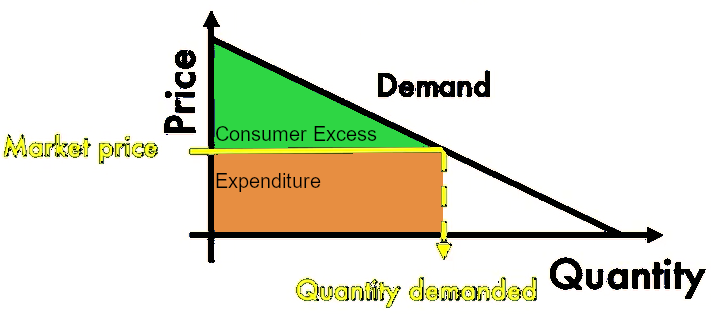
\includegraphics[width=.5\textwidth]{consumerSurplus.PNG}
  \caption{Consumer Surplus \& Expenditure}
\end{figure}

\begin{definition}{Production Costs}
  A producer will have costs they need to pay in order to stay in business. These costs can be categorised as
  \begin{itemize}
    \item[\textit{Fixed Costs}] A company must incur in order to operate, even before they start producing. (e.g. rent)
    \item[\textit{Variable Costs}] are costs which depend on the number of units produced. (e.g. equipment, raw materials)
    \item[\textit{Semi-Variable Costs}] Labour can be considered a variable cost as you can choose to pay overtime or to hire someone new in order to increase production.
  \end{itemize}
  The sum of these values will give you the \textit{Total Cost} of production.
\end{definition}

\begin{definition}{Marginal Cost Curve}
  \textit{Marginal Cost} is the cost of producing the \underline{last} unit. It is equal to
  \[ \dfrac{\text{Change in Cost}}{\text{Change in Quantity Produced}} \]
  \par We can plot a \textit{Marginal Cost Curve} of marginal cost against quantity. Typically these are initially downwards sloping, then upwards sloping.
\end{definition}

\begin{definition}{Economies of Scale}
  When the \textit{Marginal Cost Curve} is downwards sloping \textit{Economies of Scale} are being experienced. \textit{Economies of Scale} are the cost advantages a producer obtains by scaling their business. e.g. By hiring a new staff member existing staff are able to specialise better on their task and thus production per staff member increases.

  \par When the \textit{Marginal Cost Curve} is upwards sloping \textit{Diminishing Marginal Returns} are being experienced. This is common as it is unlikely that hiring 10 new staff will increase marginal production by 10 times that of a single new staff member.

  \par Economies of scale \& diminishing marginal returns affect the \textit{Cost Curve} for a producer.
\end{definition}

\begin{remark}{Minimum Sale Price}
  The \textit{Marginal Cost} of a product is the minimum price a product must be sold at in order to make a profit.

  \par A producer will go out of business if it cannot sell above its \textit{Average Variable Cost} (per unit produced) in the \underline{short run}; and if cannot cover its \textit{Average Total Cost} (per unit produced) in the \underline{long run}.

  \par The point where these \textit{AVC} \& \textit{ATC} curves intersect the \textit{Marginal Cost Curve} define the minimum amount of units a business needs to sell to stay in business in the short and long term, respectively.
\end{remark}

\begin{figure}[ht!]
  \centering
  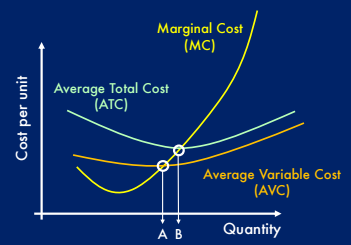
\includegraphics[width=.5\textwidth]{physicalCostCurve.PNG}
  \caption{Cost Curve for a Product of a Physcial Retailor}
\end{figure}

\begin{definition}{Business Supply Curve}
  A business's \textit{Supply Curve} is the minimum price-per-unit it is willing to sell each quantity of product at. It tends to be upwards sloping as marginal cost increases with quantity. The \textit{Supply Curve} will be truncated and not have a value for small quantities (in practice) as the business would fail if it sold too few products.
\end{definition}

\begin{definition}{Market Supply Curve}
  The \textit{Market Supply Curve} is the total number of units available, for a given price, across all producers in a market.

  \par The area above the \textit{Market Supply Curve} and below the \textit{Market Price} is the \textit{Producer Surplus}. This is the total additional income a producer receives after costs (i.e. total profit). Producers want to maximise \textit{Producer Surplus}
\end{definition}

\begin{definition}{Competitive Equilibrium}
  In a \textit{Competitive Market} the \textit{Market Equilibrium Price} will be that where the \textit{Consumer Demand Curve} and \textit{Market Supply Curve} intersect, as this is the price where quantity demanded and supplied are equal. The \textit{Market Equilibrium Price} maximises total surplus for both consumers and producers.
\end{definition}

\begin{definition}{Shifts}
  \textit{Shifts} can occur which move the whole of a supply or demand curve. These occur from non-price factors. e.g. a pandemic will cause a shift in the demand curve for face masks. These will cause a shift in  \textit{equilibrium price}.
\end{definition}

\begin{definition}{Monopoly Market}
  A market is considered a \textit{Monopoly} if its structure is characterised by a single seller (The \textit{Monopolist}). The \textit{Monopolist} faces no competition and thus can be a price \underline{setter}, rather than price taker. In the real world a firm with over 40\% market share is considered to have a monopoly. Monopoly markets are not competitive.
\end{definition}

\subsection{Elasticity}

\begin{definition}{Price Elasticity of Demand}
  \textit{Price Elasticity} is a measure of the how much the price of a product affects the quantity demanded. The more horizontal the demand curve, the greater the quantity demanded increases for a given decrease in price, (i.e. the more elastic the price is).
  \begin{itemize}
    \item A \textit{Horizontal} demand curve has \textit{Perfect Price Elasticity} as a change in quantity has no affect on price.
    \item A \textit{Vertical} demand curve has \textit{Perfect Price \underline{In}elasticity} as a fix quantity is demanded, at any price.
    \item A \textit{45 degree} demand curve has \textit{Unit Price Elasticity} as an $\Delta\%$ change in supply will produce an $\Delta\%$ change in demand.
  \end{itemize}
\end{definition}

\begin{definition}{Price Elasticity of Supply}
  \textit{Supply Elasticity} is a measure of how much a change in quantity supplied will affect the cost of production. The more horizontal the \textit{Supply Curve} is the less the price of production increases for a given quantity.
  \begin{itemize}
    \item A \textit{Horizontal} demand curve has \textit{Perfect Price Elasticity} as a change in quantity has no affect on price.
    \item A \textit{Vertical} demand curve has \textit{Perfect Price \underline{In}elasticity} as a fix quantity is demanded, at any price.
    \item A \textit{45 degree} demand curve has \textit{Unit Price Elasticity} as an $\Delta\%$ change in supply will produce an $\Delta\%$ change in demand.
  \end{itemize}
\end{definition}

\subsection{Price Discrimination}

\begin{definition}{Price Discrimination}
  \textit{Price Discrimination} is the practice of charging different prices to different customers for the same product. There are three levels of price discrimination
  \begin{itemize}
    \item[$1^\text{st}$ Degree]  \textit{Personalised} pricing. The business charges the maximum possible price for each unit sold (perfect price discrimination).
    \item[$2^\text{nd}$ Degree]  Product \textit{versioning} or \textit{menu pricing}. A company charges a different price for different quantities/qualities (ie bulk discount). Consumers have a choice over which version they buy, and thus the price.
    \item[$3^\text{rd}$ Degree]  \textit{Group} pricing. The business charges a different price to different customer groups (e.g. age,location). The consumer does not get to choose their group. The groupings try to separate customers by their \textit{price elasticity} (The more price elastic charged less).
  \end{itemize}
  See \texttt{Figure 3}

  \begin{figure}[ht!]
    \centering
    \begin{subfigure}[b]{.3\textwidth}
         \centering
         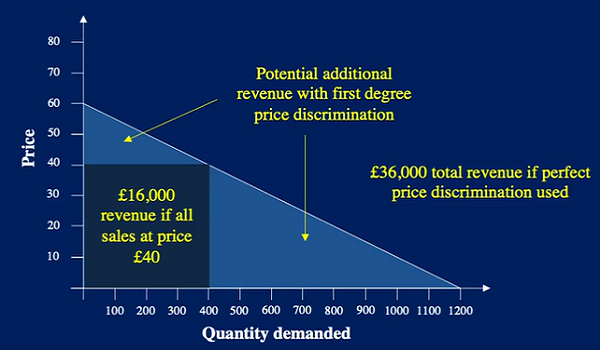
\includegraphics[width=\textwidth]{personalisedPricing.PNG}
         \caption{$1^\text{st}$ Degree}
    \end{subfigure}
    \begin{subfigure}[b]{.3\textwidth}
        \centering
        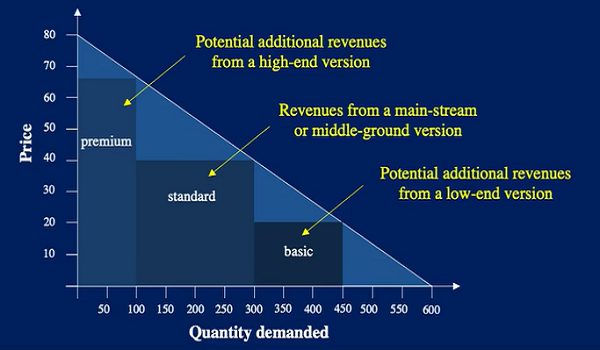
\includegraphics[width=\textwidth]{versioningPricing.PNG}
        \caption{$2^\text{nd}$ Degree}
    \end{subfigure}
    \begin{subfigure}[b]{.3\textwidth}
         \centering
         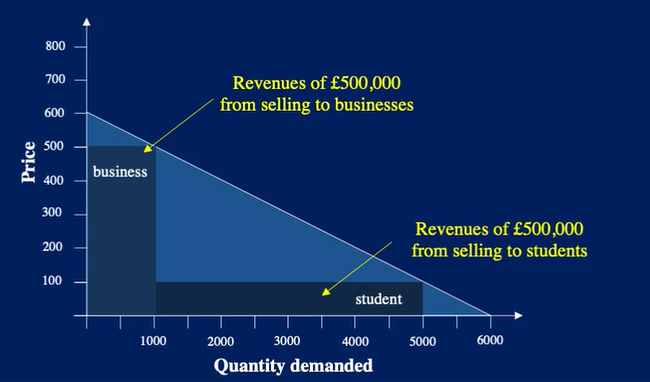
\includegraphics[width=\textwidth]{groupPricing.PNG}
         \caption{$3^\text{rd}$ Degree}
     \end{subfigure}
    \caption{Potential revenue increases for different pricing strategies}
  \end{figure}

\end{definition}

\begin{proposition}{Requirements for Price Discrimination}
  For a seller to be able to effectively price discriminate they must fulfil the following
  \begin{enumerate}
    \item Be able to \textit{distinguish between customers} so as to know what price to charge them.
    \item Have enough \textit{market power} to be able to set prices above marginal costs.
    \item \textit{Resale} must be impractical to prevent arbitrage.
  \end{enumerate}
  It is generally easier for online business to meet these criteria.
\end{proposition}

\begin{definition}{Net Utility}
  The \textit{Net Utility} of a product to a consumer is the difference between the price of the product and the consumer's perceived value of the product. (e.g. If a product is sold at £5 but a consumer values it at £7, the net utility is £7-£5=£2). It is assumed a customer will never by a product that has a \textit{negative net utility} to them.
\end{definition}

\begin{example}{Economics of Versioning}
  Suppose we have a product priced at £10. Consider two customers: \textit{addict} who values it at £20; and \textit{casual} who values it at £8. The company will sell a single unit (to \textit{addict}) at £10.
  \par Now, suppose the company brought in a \textit{cut-down} version at £5 which \textit{addict} values at £8; and the casual user at £7. The company will now sell one full product (to \textit{addict}) and one \textit{cut-down} product (to \textit{casual}) for a total of £15.
  \par In fact, pricing the \textit{cut-down} version at £7 and the \textit{full} version at £19 would maximise profit (assuming customers go for the superior product when they have the same net utility for both) as this would be a perfect price for  \textit{casual} and the net utility is the same (£1) for \textit{addict} for both products.
\end{example}

\begin{proposition}{Competing against Yourself}
  A risk of versioning is that consumers who are willing to pay for the higher price, will choose to pay for the lower price one (due to greater net-utility). Thus choosing pricing points \& functionalities is therefore critical to business success.
\end{proposition}

\begin{proposition}{Bundling}
  \textit{Bundling} is a form of \textit{versioning} where several goods are sold together for a single price. (e.g. microsoft office). Bundling is used to sell customers products they would not otherwise buy. Bundling can create barries to entry for competitor producers as it requires competitors to produce a wider varity of product (e.g. a spreadsheet software \& word processor rather than just one).
\end{proposition}

\section{The Economics of The Internet}

\begin{definition}{Network Externalities}
  A \textit{Network Externality} is an \textit{Externality} that occurs when the act of buying a product/serivce has an indirect cost or benefit to those who already own the same product/service. Products with \underline{positive} network externalities are often known as \textit{Network Goods}.

  \par Owning a mobile phone has a positive network externality as you are increasing the number of contactable people. Owning a car has a negative network externality as you increase road traffic.

  \par Positive network externalities can produce a \textit{Positive Feedback Loop} where people by products which are compatible with their friends, rather than necessarily the best product. This is part of \textit{Brand Value}.
\end{definition}

\begin{definition}{Network Effect Demand Curve}
  We can plot a \textit{Network Effect Demand Curve} (\texttt{Figure 3}) of the price customers are willing to pay against network size. This is slope upwards initially as the marginal value of each extra user is higher; eventually it will slope downwards as these marginal gains diminish.

  \par For any given price there are three equilibrium points $q_0,q_1,q_2$ for network size. $q_1$ is deemed unstable, the \textit{`tipping point'}, as once the network is larger than $q_1$ it will naturally grow to $q_2$ (as there is a consumer excess) but whilst it is smaller it will shrink to $q_0$ (as there is a consumer deficit). This means $q_1$ is the \textit{Critical Mass} for the network to be sustainable.
\end{definition}

\begin{figure}[ht!]
  \centering
  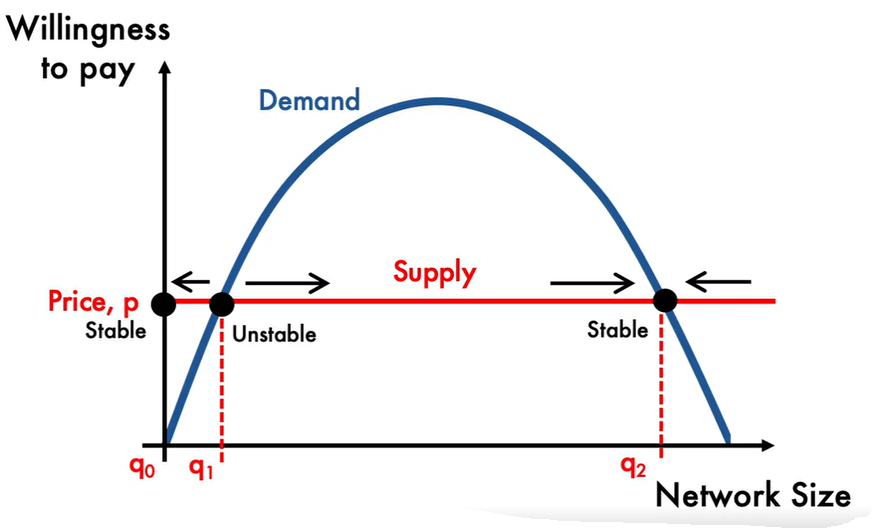
\includegraphics[width=.5\textwidth]{networkDemandCurve.PNG}
  \caption{Network Effect Demand Curve}
\end{figure}

\begin{proposition}{The Long Tail}
  Sales business typically sell either: high volume, low margin goods (e.g. burgers); Or, low volume, high margin goods (e.g. cars). Physcial sales businesses are constrained by the physical shelf space they have and thus avoid low volume, low margin goods. This means that the sales distribution for products in a physical store will be a truncated \textit{Pareto Distribution}.\\
  \par Internet businesses have unlimited shelf space to advertise products, and since warehouse space is much cheaper (per sq ft) they can store a lot more products for the same cost, effectively increasing the margin of each product. Meaning their are more products which are profitable to stock and the sales distribution for products of an internet business will have a much longer tail. (See \texttt{Figure 1}).
\end{proposition}

\begin{figure}[ht!]
  \centering
  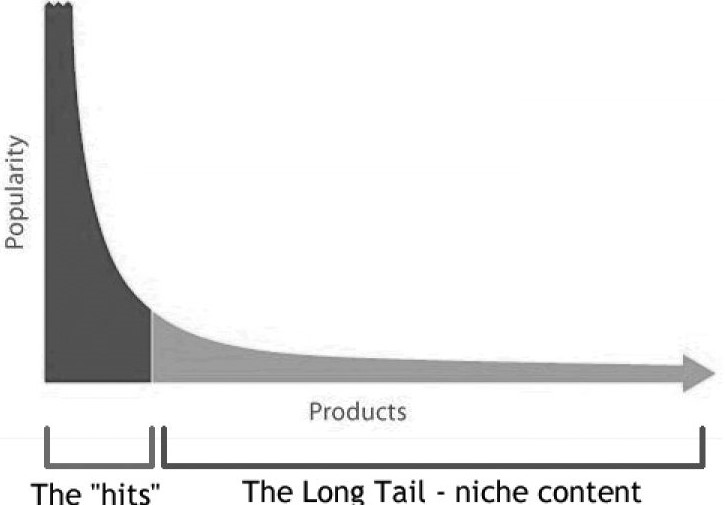
\includegraphics[width=.5\textwidth]{LongTail.jpg}
  \caption{The Long Tail}
\end{figure}

\begin{remark}{How to take advantage of `The Long Tail'}
  \begin{enumerate}
    \item Make everything available.
    \item Reduce prices (due to economies of scale \& reduced costs).
    \item Help customers find new products.
  \end{enumerate}
\end{remark}

\begin{remark}{Sustaining v. Disruptive Innovations}
  \textit{Sustaining Innovations} are those that incrementally improve existing products on traditional performance metrics. Eventually these will superceed customer requirements.
  \par \textit{Disruptive Innovations} perform less well on traditional performance metrics but sufficiently better along other metrics in order to generate new markets.
\end{remark}

\begin{proposition}{Disruptive Technology}
  Established companies are often late to invest in new \textit{disruptive} technologies. Typically this is due to the \textit{disruptive} tech not reaching the requirements of their customers. However, the \textit{disruptive} tech maybe better in other ways (lighter, more durable etc.) and so can establish a sufficient market for startups to invest in it. Once the \textit{disruptive} tech does reach the requirements of mainstream customers, they are likely to jump to the new tech for these bonus features (lighter, more durable etc.) and the established company may fail.
  \par The new tech may still be less powerful than the established tech, but it is sufficient for customers so it doesn't matter. The traditional performance metric for performance will vary by industry (e.g. mb/£ for hard drives).
\end{proposition}

\begin{proposition}{Timeline of Disruptive Technology}
  \begin{enumerate}
    \item \textit{Disruptive Technology} is invent. Often by an established company.
    \item The \textit{disruptive technology} does not meet established the established company's requirements and so not focused on.
    \item New companies form to pursue the \textit{disruptive technology}. Often by ex employees of the established company.
    \item \textit{Disruptive Technology} improves \& meets traditional performance metric requirements. The established company will likely try to enter the new market at this point but will be too late.
    \item \textit{Disruptive Technology} becomes the main stream.
  \end{enumerate}
\end{proposition}

\begin{proposition}{How to spot Disruptive Technology}
  \begin{enumerate}
    \item \textit{Determine whether the technology is disruptive or sustaining}
  \end{enumerate}
\end{proposition}

\subsection{Properties of Online Businesses}

\begin{remark}{Economic Laws}
  The \textit{Economic Laws} are not fundamentally different between online \& irl businesses, but the characteristics of online business activities can result in different markets.
\end{remark}

\begin{definition}{Combinatorial Innovation}
  \textit{Combinatorial Innovation} describes a technology who's components can be combined \& recombined to create new products and services. The Internet is a \textit{Combinatorial Innovation} due to its standardised and open-source nature.
\end{definition}

\begin{proposition}{Economic Differences between Digital \& Physical Goods}
  \begin{itemize}
    \item Digital goods tend to be costly to produce; but \textit{cheap to reproduce}. (i.e. Fixed costs are high but variable costs are low).
    \item Production costs for digital goods are \underline{sunk} costs. (e.g. You can sell a building you don't need, but cannot get money back from a software developer).
    \item There are \textit{no capacity constraints} limiting the number of times something can be reproduced.
    \item Digital goods are often \textit{Experience Goods}. (i.e. a customer will no know whether they will like it before they try it, and thus cannot assign a value to it).
    \item \textit{Serach Costs} for a consumer are very low. It is easy for consumer to compare products are go with the best. IRL this is harder as it requires going to different stores.
    \item Digital goods have \textit{strong positive network externalities}
  \end{itemize}
\end{proposition}

\begin{remark}{Switching Costs}
  A customer may incur a cost (inc. non-monetary) to switch services. This is more common (and costly) in the digital space than the physical. When switching costs are too high, consumers are \textit{locked in}. Possible switching costs include:
  \begin{itemize}
    \item Training cost.
    \item Network effects.
    \item Setup costs.
    \item Reduced service quality due to new provider not having all your information (consider switching from Netflix).
  \end{itemize}
\end{remark}

\begin{proposition}{Cost Curve for Digital Goods}
  Since digital goods have high fixed cost but low variable costs their \textit{cost curves} are very different. The \textit{Marginal Cost Curve} is effectively zero for all quantities; Average Variable Costs are effectively zero for all quantities; and, average total costs tend asymptotically towards zero.
  \par This means it is easy for an online business to survive in the short term and the minimum price they are willing to sell a product at is zero (due to v. low variable costs). Eventually the company will need to pay off its fixed costs.
\end{proposition}

\begin{figure}[ht!]
  \centering
  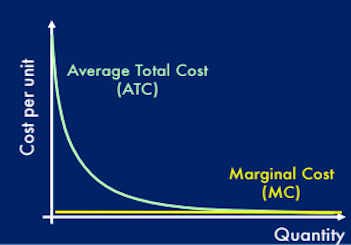
\includegraphics[width=.5\textwidth]{digitalCostCurve.PNG}
  \caption{Consumer Surplus \& Expenditure}
\end{figure}

\begin{remark}{Competition between Digital Companies}
  \begin{itemize}
    \item Due to low variable costs, companies with identical digital products will very quickly move prices to near-zero.
    \item New companies will struggle as fixed costs are high.
    \item Network effects \& switching costs make it hard for new companies.
  \end{itemize}
  Due to these \textit{barriers to entry} monopolies are common among digital companies. To succeed, a company needs to focus on product differentiation (i.e. innovation).
\end{remark}

\begin{remark}{Formats}
  Companies can make their software use \textit{Proprietary Formats}, meaning the files cannot be used by other software. This increases switching costs for customers.
  \par Using \textit{Industry-Wide Standards} allow a user's files to be shared between providers. This can increase the network effect, potentially attracting new customers. Here companies have a trade-off between having a large part of a small pie, or a small part of a large pie.
\end{remark}

\begin{remark}{How Standards Develop}
  \textit{Industry-Wide Standards} general develop in one of two ways
  \begin{enumerate}
    \item A \textit{single (major) player} sets a standard by opening up their proprietary format (e.g. PDF).
    \item A \textit{war} occurs between multiple standard setters. Generally detrimental to everyone involved.
    \item A \textit{negotiation} occurs between multiple standard setters. There is a risk that one party may pull out of the deal and use their own proprietary format.
  \end{enumerate}
\end{remark}

\subsection{Price Discrimination Online}

\begin{remark}{Personalised Pricing Online}
  \begin{itemize}
    \item Consumers tend perceive personalised pricing as \textit{unfair}.
    \item Consumers like \textit{transparency} (i.e. how a price is decided).
    \item European data protection laws \textit{require} companies inform people about the specific purpose of processing their personal data.
  \end{itemize}
\end{remark}

\begin{proposition}{Digital Product Versioning}
  \begin{itemize}
    \item Digital versions are used extensively and creatively as they are easy to prepare and near-zero cost to duplicate.
    \item Buyers have a choice over which version to buy, so do not find the practice controversial.
    \item \textit{Personalisation of Product} is an extreme typr of product versioning (becoming closer to $1^\text{st}$ degree price discrimination) as it allows user to specify many properties (e.g. screen quality, amount of ram \& storage for a pc).
    \item People tend to \textit{upsell} towards an ``almost top option'' when given a choice (the 2nd most expensive bottle of wine is often the most popular).
    \item Product versioning can cause you to \textit{compete with yourself} as some people who would have payed the higher price, will go for the lower price.
  \end{itemize}
\end{proposition}

\begin{remark}{Unbundling}
  \textit{Bundling} is common with physical software but there is also a practice of \textit{unbundling}. Since there is no physical substrate online there is less commercial pressure to bundle. (e.g. publishers can sell individual articles rather than a full magazine).
\end{remark}

\begin{remark}{'Free' Digital Versions}
  As the duplication cost of digital goods is almost zero, many are given away for free. In these cases there are still several ways for producers to make money: cut-down versions encourage you to buy a full version; Artificial delay (e.g. stock feeds); Ads (or pay for no adds).
  \par \textit{'Free'} versions allow a customer to build a truer valuation of a product, particularly useful for \textit{experience goods}.
  \par Even if a user is on the free model they are building the \textit{network effect} of the product and likely increasing the \textit{swapping costs} they will experience if they want to change product.
\end{remark}

\begin{proposition}{Freemium Model}
  The \textit{'Freemium'} business model is to offer different versions at different prices, \textit{including a free one}. The hope is a consumer will \textit{upgrade} to a paid version because they like the service.
\end{proposition}

\section{Auction Theory}

\begin{remark}{Why Use Auctions?}
  \textit{Auctions} allow an item to be sold for a price which is wholely decided by a consumer's willingness to spend. \textit{Auctions} are a mechanism for first-degree \textit{price discrimination}, this makes them particulary popular online.
  \par Auctions are used when sellers are \textit{uncertain} about the value consumers place on an object (common with one off items). In this case auctions are good as they allow for \textit{price discovery}.
  \par Auctions are easy to automate and a form of differential pricing.
\end{remark}

\begin{proposition}{Auctions vs Posted Prices}
  When a seller chooses to run either an auction or use posted prices, they are choosing whether between \textit{price discovery} and \textit{convenience}. Auctions are often favoured by unexperienced sellers and unique items. Auctions sell for less than a posted price listing (otherwise consumers would pay the posted price listing).
\end{proposition}

\begin{definition}{Private Value}
  An object's \textit{Private Value} is the value each consumer places on the object. Each bidder knows their private value for an object, but do not know the private value of others nor does knowledge of other bidders' private values affect your private value. This situation is common for consumable goods, less so with investments.
\end{definition}

\begin{definition}{Interdependence}
  \textit{Interdependence} occurs when a bidder does know have a fixed value for an object and use other bids to improve their estimate of an objects value. This is common when other bidders may have more information.
\end{definition}

\begin{definition}{Open Auction}
  In an \textit{Open Auction} all bids are known to all particpants.
\end{definition}

\begin{remark}{Assumptions in Auction Theory}
  In Auction theory several assumptions are made:
  \begin{itemize}
    \item All auctions are equally attractive (ie there are no auctions where no one turns up);
    \item There is no collusion between bidders;
  \end{itemize}
  These assumptions means auction theory often does not work well in practice.
\end{remark}

\begin{remark}{Attendance at Auctions}
  Entering an auction can be quite involved, so often bidders will skip auctions they don't think they can win.
\end{remark}

\begin{definition}{Signalling}
  During an auction a bidder may place a \textit{`weird`} bid which signals their intent for the rest of the auction to other bidders. This is a form of collusion without any prior agreement necessary. (Consider the T-Mobile - Mannesbane auction for parts of the german telephone network).
\end{definition}

\begin{definition}{Reverse Auction}
  \textit{Reverse Auctions} are when multiple suppliers bid for a contract with a single consumer. This is commonly used for construction \& suppliment contracts, (inc. by governments).
  \par Often suppliers must be \textit{qualified} in order to \textit{offer} a price.
\end{definition}

\begin{definition}{Double Auction}
  In a \textit{Double Auction} multiple buyers and multiple sellers take part. The sellers offer descending prices, and buyers bid ascending prices. When two prices meet a sale is made between those two parties.
  \par \textit{Continuous Double Auctions} all buyers and sellers to place bids at any time, and not necessarily in order. This is used in stock exchanges.
  \par \textit{Double Auctions} are very efficient for price discovery.
\end{definition}

\begin{proposition}{Trading in the Dark}
  Sometimes you do not want to give away your private information (e.g. You dont want to list a large stock sale on a public order book as this would affect the stock price).
  \par \textit{Dark Pools} are designed to keep your trading intensions secret so that it does not impact price. WARNING it is common for dark pool owners to use this information against their users.
\end{proposition}

\subsection{Open Auctions}

\begin{definition}{English Auction}
  AKA \textit{Open Ascending-Price Auction}. Used in \textit{Homes under the Hammer}.
  \begin{enumerate}
    \item The auctioneer announces a (low) price to everyone.
    \item If a bidder is happy to pay that price they raise their hand. (Price is reduced if no one bids).
    \item Auctioneer will announce that that bidder is currently winning and will announce a new, higher price.
    \item ii)-iii) repeat until no-one accepts the new higher price (ie no hands are raised)
    \item The item is sold to the person who bid last, at the price of that last bid.
  \end{enumerate}
  Bidders can infer information from when others drop out of an auction. However, with \textit{Private Values} this will not change their strategy (it would for \textit{Interdependence}).
\end{definition}

\begin{proposition}{English Auction - Optimal Strategy}
  Let $v$ be the private value a bidder assigns to an object
  \begin{itemize}
    \item It is not optimal for a bidder to bid a price $p$ if $p>v$ as the bidder makes a loss.
    \item It is not optimal for a bidder to drop out at a price $p<v$ as the bidder still has surplus demand.
  \end{itemize}
  Therefore, the optimal strategy is to bid on any price $p$ that does not exceed $v$.
\end{proposition}

\begin{remark}{Weak Bidders}
  It is harder for a weak bidder to win an English auction as stronger bidders can just accept the next price.
\end{remark}

\begin{definition}{Dutch Auction}
  AKA \textit{Open Descending-Price Auction}. Used in \textit{Dutch Flower Markets}.
  \begin{enumerate}
    \item The auctioneer announces a (high) price to every.
    \item The auctioneer keep reducing the price until someone bids (raises their hand).
    \item The item is sold to this (first) bidder, at the price the auction was stopped.
  \end{enumerate}
\end{definition}

\begin{proposition}{Dutch Auction - Optimal Strategy}
  Shade you bid. i.e. bid $p<v$ where $v$ is your private value.
\end{proposition}

\begin{remark}{Robustness}
  Collusion is much easier in an open auction, meaning the auction is less robust.
\end{remark}

\subsection{Sealed Auctions}

\begin{definition}{Sealed Auction}
  In a \textit{Sealed Auction} bidding is done in private. Participants do not know what others have bid.
\end{definition}

\begin{definition}{First-Price Sealed Bid Auction}
  Used to buy \textit{Houses in Scotland}.
  \begin{enumerate}
    \item Auctioneer announces the auction is open and how long it is open for.
    \item Each participant makes a single secret bit.
    \item The highest bid will win, and will pay that price. (ie pay \textit{First-Price})
  \end{enumerate}
\end{definition}

\begin{proposition}{FPSB - Optimal Strategy}
  Shade you bid. i.e. bid $p<v$ where $v$ is your private value.
\end{proposition}

\begin{definition}{Second-Price Sealed Bid}
  AKA a \textit{Vickery Auction}
  \begin{enumerate}
    \item Auctioneer announces the auction is open and how long it is open for.
    \item Each participant makes a single secret bit.
    \item The highest bid will win, and will pay the price of the second highest bid. (ie pay \textit{Second-Price})
  \end{enumerate}
\end{definition}

\begin{proof}{SPSB Auction - Optimal Strategy}
  Let $v$ be the private value a bidder assigns to an object, $p$ be the value they bid and $c$ be the greatest value of a competitor bid.
  \par If $p=v$ then
  \begin{itemize}
    \item Bidder wins if $c<p=v$ for a profit of $(v-c)$.
    \item Does not win if $v=p<c$.
  \end{itemize}
  If $p<v$ then
  \begin{itemize}
    \item if $v>p>c$ then the bidder \textit{still} wins with profit $v-c$.
    \item if $c>v>p$ then the bidder \textit{still} loses.
    \item if $v>c>p$ then the bidder \underline{now} loses (making less profit), where they wouldn't have with the previous strategy.
  \end{itemize}
  Therefore, bidding $p<v$ never increases a bidders profit. A similar argument can be made for not bidding $p>v$.\\
  The optimal strategy is to bid $p=v$ (same as an \textit{English Auction})
\end{proof}

\begin{remark}{Auctions for Sellers}
  If buyers are risk averse (ie don't want to lose the opportunity of buying) then FPSB can increase revenues over SPSB auctions.
\end{remark}

\begin{remark}{Robustness}
  Sealed auctions are more robust as you cannot observe other bidders actions, and thus cannot punish a colluder who defects.
\end{remark}

\begin{remark}{Weak Bidders}
  Weak Bidders have a better chance of winning a sealed auction as other bidders may over-shade their bid.
\end{remark}

\subsection{Equivalent Auctions}

\begin{definition}{Incentive Compatible}
  Auctions are \textit{Incentive Compatible} if they encourage bidders to bid their true value for an item. Incentive compatible auctions stop game playing between bidders as there is no advantage to second guess other users' values. This makes \textit{Incentive Compatible} auctions more predictable and thus favourable for auctioneers.
  \par English \& SPSB auctions are incentive compatible.
\end{definition}

\begin{remark}{Equivalence of English \& Second-Price Sealed Bid Auctions}
  English \& SPSB auctions are weakly equivalent as the optimal strategies are only the same if values are \textit{private} (i.e. there is no \textit{interdependence}).
\end{remark}

\begin{remark}{Strategic Equivalence of Dutch \& First-Price Sealed Bid Auctions}
  Bidding a certain amount in a FPSB auction is equivalent to offering to buy at that amount in a Dutch auction. Thus they are \textit{Straegically Equivalent} (for all strategies in one game there is a strategy in the other which will produce the same outcome).
\end{remark}

\begin{theorem}{Revenue Equivalence Theorem}
  If private values are iid and all bidders are risk neutral, then any standard auction yields the same expected revenue to the seller.
\end{theorem}

\begin{remark}{Revenue Equivalence Theorem}
  In practice the \textit{Revenue Equivalence Theorem} does not hold since bidders are not risk neutral (they do have an emotional attachment to goods) and interdependence exists.
\end{remark}

\subsection{Online Auctions}

\begin{remark}{Auctions Online}
  Due to the algorithmic nature of auction rules \& no need for a physical auctioneer or room, the internet enables auctions to be run quickly and cheaply.
  \par Bidding can be automated too, and more complex auction rules can be implemented.
  \par The only limit to online auctions is server capacity and bandwidth.
\end{remark}

\begin{remark}{Intermediates}
  In the beginning of the Internet it was believed that small businesses (e.g. farmer) would be able to sell to customers directly, without the need of an intermediary (e.g. supermarket). This has not been realised as it is much harder to get customers attention online. So \textit{Online Marketplaces} (e.g. amazon, ebay) sprung up to act as intermediaries.
  \par Online marketplaces not host listings but also ease payments and improve trustworthiness of both sellers \& buyers.
\end{remark}

\begin{remark}{eBay}
  \textit{eBay} is one of the most famous online auctioneers. Mainly does consumer-to-consumer and business-to-consumer auctions, but also some business-to-business.
  \par Reviews of sellers act as a lock-in mechanism and part of why \textit{eBay} has an effective monopoly.
  \par eBay auctions are open-ascending auctions with a deadline set before the auction begins (similar to an english auction, but with a time line).
\end{remark}

\begin{remark}{Snipping}
  The timelimit on eBay auctions has lead to phenomena of \textit{snipping}, where bidders wait to place their bid till near the end of an auction in the hope it is too late for anyone else to join (and so as not to give away information about their value).
  \par eBay don't like this as there is hidden information.
  \par To combat this eBay introduced a `proxy' bidding functionality (if everyone uses this then it is similar to a SPS auction). Alternatively, they could have extended the time limit each time someone bid (similar to a true english auction)
\end{remark}

\begin{proposition}{Estimating Demand for Dynamic Pricing in Electronic Markets}
  \begin{enumerate}
    \item Track bidders and \textit{`recover`} missing bidders (who could not bid as the price was too high when they first entered). Use this data to estimate a demand curve.
    \item Build a demand and supply curve.
    \item Calculate supplier costs and estimate revenues.
    \item Determine optimal sales quantity/strategy using the revenue and cost curves.
  \end{enumerate}
\end{proposition}

\begin{remark}{Google Ad Auctions}
  Google understands their customer very well as they know exactly what they are looking for. Adverts for webpages are highly idiosyncratic and thus hard to compare.
  \par Google uses auctions on its ad-space in order to perform price discovery. Multiple auctions are done for each user search (~60k auctions per second). Google considers both the \textit{bid price} and the \textit{advert quality} when choosing the winner of an auction, as they don't want their users to get loads of shit adds.
  \par \textit{Advert quality} is assessed using: Historic click-through-rate; relevancy; and landing page quality (inc. load speed).
  \par This type of auction works best for the seller when there is lots of competition in the auction. To encourage this Google relax the strictness of their keyword matching.
  \par Originally, Google used FPSB auctions but this lead to their servers being overloaded with advertisers checking the results of auctions (to see if they could lower their price). Google then switch to SPSB auctions, solving the server overload problem, as this is \textit{incentive compatible}.
\end{remark}

\end{document}
